date : 9 januari 2024

Data communicatie:\\
simplex: van A naar B\\
Half -duplex: van A naar B of B naar A\\
Full-duplex: Van A naar B en B naar A.

Een synchroom signaal stuur ook een referentie klok mee.

\subsubsection{I2C}
\begin{itemize}
    \item two wired bus: SDA (data) en SCL (clock) <- (dus synchroom)
    \item originally to interact within small numbers of chips
    \item speeds:
    \begin{itemize}
        \item 100 kbps (standard mode)
        \item 400 kbps (fast mode)
        \item 3.4 Mbps (high-speed mode)
    \end{itemize}
    \item data transfer: serial, 8-bit oriented, bi-directional (Half-duplex)
    \item master/slave relationship wiht multi-master option
    \item master can operate as transmitter or receiver
    \item addressing: 7 bit or 10 bit unique addresses
    \item device count limit : max. capacitance 400pF
\end{itemize}

\begin{figure}[H]
    \centering
    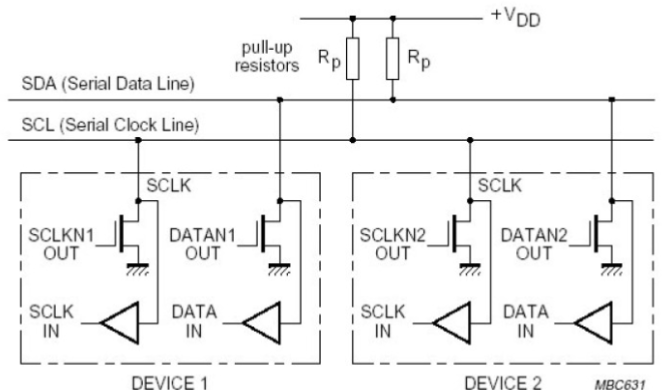
\includegraphics[scale=0.7]{i2c.png}
    \caption*{ I2C}
    \end{figure}

\begin{figure}[H]
    \centering
    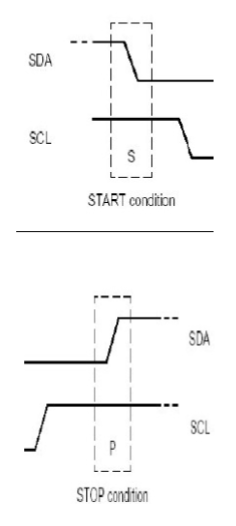
\includegraphics[scale=0.7]{i2c start stop.png}
    \caption*{start stop signaal van I2C}
    \end{figure}

\begin{figure}[H]
    \centering
    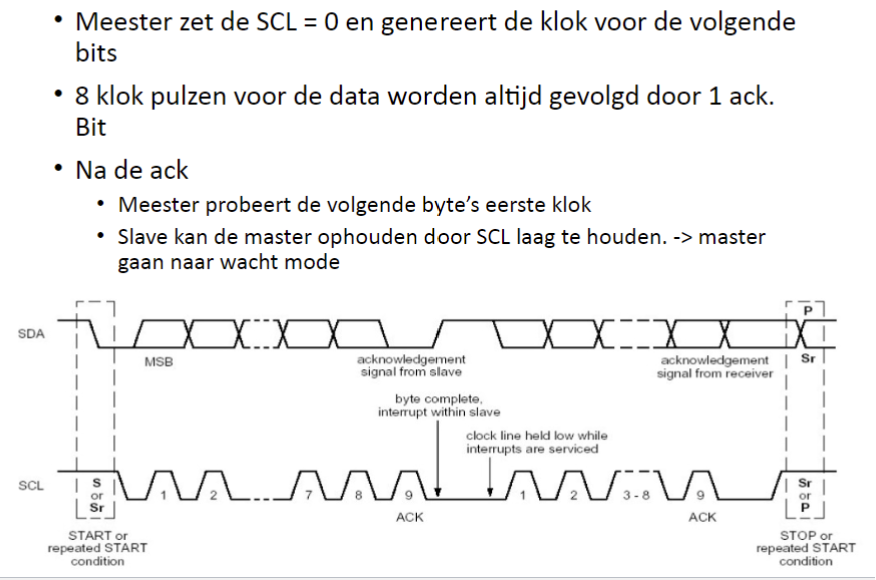
\includegraphics[scale=0.7]{Data transfer i2c bus.png}
    \caption*{Data transfer I2C bus}
    \end{figure}

Bij de 9de scl puls moet de slave de sda laag houden om te acken. Slave moet SDA ook weer loslaten na de ack
(neergaande klok).

\begin{figure}[H]
    \centering
    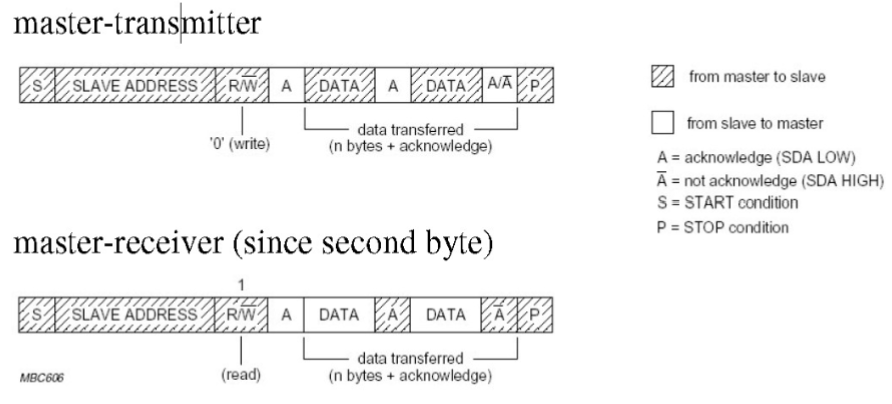
\includegraphics[scale=0.7]{Frame Format.png}
    \caption*{Frame format van I2C}
    \end{figure}

\subsubsection{1-Wire}
\begin{figure}[H]
    \centering
    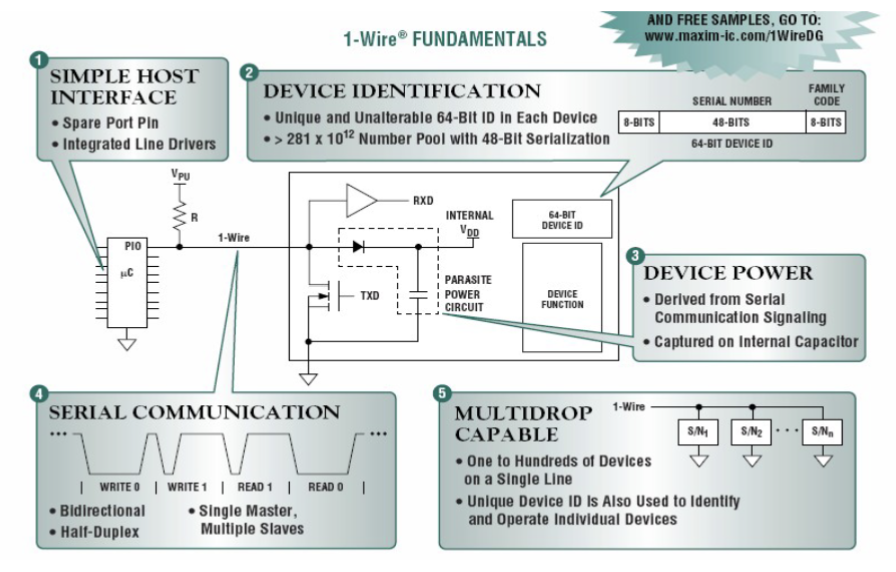
\includegraphics[scale=0.7]{1wire fundemental.png}
    \caption*{1-Wire Fundementals}
    \end{figure}

Wat is 1-wire?
\begin{itemize}
    \item Low-cost micro Lan.
    \item Digital communicatie over twisted pair
    \item globale opbouw.
    \begin{itemize}
        \item Open drain master/slave multidrop
        \item max 1 master
        \item Slave, dus 'spreek meester' en dan pas antwoorden.
        \item communicatie tussen slaves alleen mogelijk via de master.
    \end{itemize}
    \item trager dan I2C maar wel grotere afstanden <100m
    \item Standaard mode 15kbps in onverdrive 111kbps
\end{itemize}

\vspace{0.5cm}
Eigenschappen protocol
\begin{itemize}
    \item 64 bit uniek addresses8x8 bits
    \item start met LSB
    \item Eersste 8 bits familie code en identificatie
    \item Volgende 6*8 bits vormen een uniek nummer
    \item Laatste  bits is een CRC van de 1e byte ter verificatie
    \item aantal adressen dus 2 tot de macht 48 zijn er heel veel.
\end{itemize}

\begin{figure}[H]
    \centering
    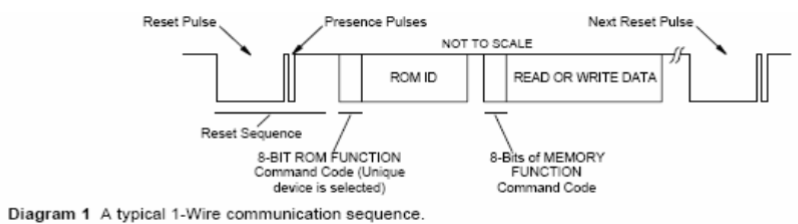
\includegraphics[scale=0.7]{1wire communicatie.png}
    \caption*{1-Wire communication}
    \end{figure}

\subsubsection{SPI van Motorola}
\begin{itemize}
    \item Geen protocol op de lijn
    \item In vergelijk met I2C snel
    \item synchroomMaster nodes in chipsFull duplex mogelijk
    \item adresseren met de slave select
\end{itemize}

Inerface bestaat uit:\\
SCLK: de klok.\\
MOSI: van de master naar de slave.\\
MISO: van de slave naar de master.\\
SSC of SS: Slave select.

\subsubsection{AMBA Bus}
\begin{figure}[H]
    \centering
    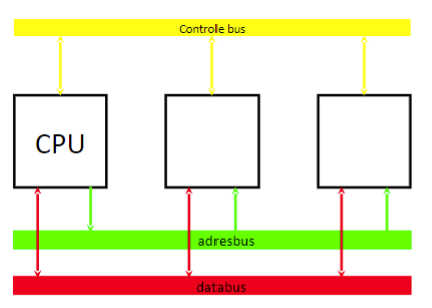
\includegraphics[scale=0.7]{AMBA bus.png}
    \caption*{AMBA Bus}
    \end{figure}

AMBA Bus wordt gebruikt voor SoC's. SoC's zijn system on chip designs overterwijl chip+software+integration.

\vspace{0.5cm}
AMBA (Advanced Microcontroller Bus Architecture) is a collection of buses from ARM for stisfying a range of different criteria.

APB (Advanced Peripheral Bus): simple strobed-acces bus with minimal interface complexity. Suitable for hosting peripherals.
\begin{itemize}
    \item Is geoptimaliseerd voor minimale vermogensopname
    \item Vereendvoudige opbouw van het businterface
    \item Relatieve lage bandbreedte t.o.v. de AHB of ASB
    \item Geen piplined operations
    \item Nieuwste versie APB relateert alle operaties t.o.v. de opgaande flank
    \item lage belasting AHB of ASB door toepassing van een APB bridge
\end{itemize}

ASB (Advanced System Bus): a multimaster synchronous system bus.

AHB (Advanced High Performance Bus): a high- throughput
synchronous system backbone. Burst transfers and split transactions.
\begin{itemize}
    \item 4 logische elementen:
    \begin{itemize}
        \item master
        \item slave
        \item arbitter
        \item decoder
    \end{itemize}
    \item meerdere busmasters
    \item split transactions :Een slaafje met een lange response tijd kan tijdens het decoderen van de opdracht de bus
    loslaten en een ander proces laten passeren. Hierna is het tijd voor het eerste slaafje als hij zijn
    werkje klaar heeft
    \item single clock edge operation: Heel handig wanneer je timing analyse aan de gang gaat. Hiermee is het mogelijk om je ontwerp
    te controleren en te verifiëren
    \item non-tristate implementation: Gebruik van een centrale gemultiplexte bus.
    \item variable bus bredte 16,32,64,128 bits
\end{itemize}

• One solution to the design productivity gap is to make ASIC designs
more standardized by reusing segments of previously manufactured
chips.

• These segments are known as “blocks”, “macros”, “cores” or “cells”.

• The blocks can either be developed in-house or licensed from an IP
company.

• Cores are the basic building blocks

• Voorbeeld: de cc2430 zigbee chip.

The principle drawbacks of SoC design are associated
with the design pressures imposed on today’s
engineers , such as:
\begin{itemize}
    \item Time-to-market demands
    \item Exponential fabrication cost
    \item Increased verification requirements
    \item Increased system complexity
    \item Design Gap
\end{itemize}

\begin{figure}[H]
    \centering
    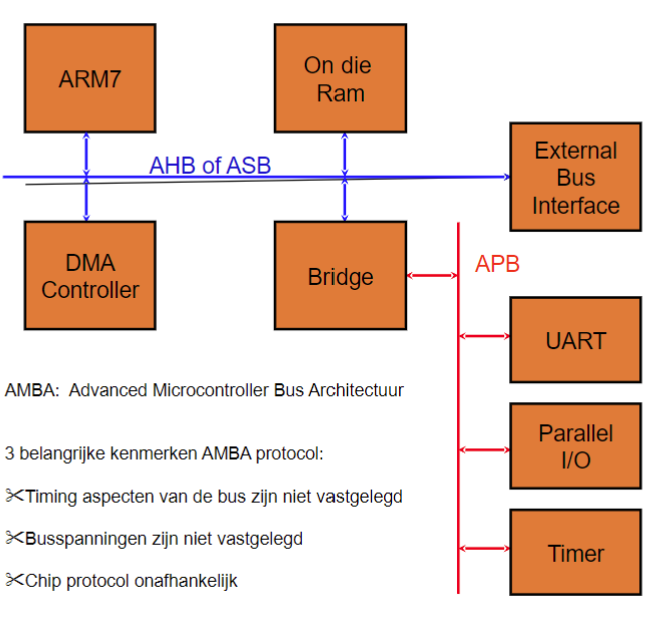
\includegraphics[scale=0.7]{amba.png}
    \end{figure}

\vspace{1cm}

Bus conclusie:\\
AHB gebruiken we als systeembus wanneer een hoge bandbreedte vereist is tussen de macrocellen en de arm processor.\\
ASB is de systeembus voor de midrange toepassingen of de oude arm processors.\\
APB is een aparte bus die men gebruikt als interface naar peripherals met een lage bandbreedte welke geen gebruik maken van pipelining



